\documentclass[11pt]{article}
\usepackage{lmodern}
\usepackage{amssymb,amsmath}
\usepackage{ifxetex,ifluatex}
%\usepackage{fixltx2e} % provides \textsubscript
\usepackage{xr} % referencing external ducument
\ifnum 0\ifxetex 1\fi\ifluatex 1\fi=0 % if pdftex
  \usepackage[T1]{fontenc}
  \usepackage[utf8]{inputenc}
\else % if luatex or xelatex
  \ifxetex
    \usepackage{mathspec}
  \else
    \usepackage{fontspec}
  \fi
  \defaultfontfeatures{Ligatures=TeX,Scale=MatchLowercase}
\fi
% use upquote if available, for straight quotes in verbatim environments
\IfFileExists{upquote.sty}{\usepackage{upquote}}{}
% use microtype if available
\IfFileExists{microtype.sty}{%
\usepackage{microtype}
\UseMicrotypeSet[protrusion]{basicmath} % disable protrusion for tt fontshttps://de.overleaf.com/project/5e85b0680d0bed00011ea790
}{}
\usepackage[margin=1in]{geometry}
\usepackage{hyperref}
\hypersetup{unicode=true,
            pdftitle={Title: Limitations to the Human Neandertal Admixture dating Supplements},
            pdfauthor={Leonardo Nicola Martin Iasi (Max Planck Institute for Evolutionary Anthropology, MPI EVA), Dr.~Benjamin Marco Peter (MPI EVA, benjamin\_peter@eva.mpg.de)},
            pdfborder={0 0 0},
            breaklinks=true}
\urlstyle{same}  % don't use monospace font for urls
 
\usepackage{natbib}
\bibliographystyle{References/my_abbrvnat}
\setcitestyle{authoryear,open={(},close={)}}

\usepackage{graphicx,grffile}
\makeatletter
\def\maxwidth{\ifdim\Gin@nat@width>\linewidth\linewidth\else\Gin@nat@width\fi}
\def\maxheight{\ifdim\Gin@nat@height>\textheight\textheight\else\Gin@nat@height\fi}
\makeatother
% Scale images if necessary, so that they will not overflow the page
% margins by default, and it is still possible to overwrite the defaults
% using explicit options in \includegraphics[width, height, ...]{}

\setkeys{Gin}{width=\maxwidth,height=\maxheight,keepaspectratio}
\IfFileExists{parskip.sty}{%
\usepackage{parskip}
}{% else
\setlength{\parindent}{0pt}
\setlength{\parskip}{6pt plus 2pt minus 1pt}
}
\setlength{\emergencystretch}{3em}  % prevent overfull lines
\providecommand{\tightlist}{%
  \setlength{\itemsep}{0pt}\setlength{\parskip}{0pt}}
\setcounter{secnumdepth}{0}
% Redefines (sub)paragraphs to behave more like sections
\ifx\paragraph\undefined\else
\let\oldparagraph\paragraph
\renewcommand{\paragraph}[1]{\oldparagraph{#1}\mbox{}}
\fi
\ifx\subparagraph\undefined\else
\let\oldsubparagraph\subparagraph
\renewcommand{\subparagraph}[1]{\oldsubparagraph{#1}\mbox{}}
\fi



\usepackage{setspace}
\onehalfspacing
\usepackage[left]{lineno}
\linenumbers
\usepackage[none]{hyphenat}
\usepackage{amsfonts}
\usepackage{amssymb}
\usepackage{graphicx}
\usepackage{float}
\usepackage{xcolor}
\usepackage{booktabs}
\usepackage{longtable}
\usepackage{array}
\usepackage{multirow}
\usepackage{wrapfig}
\usepackage{float}
\usepackage{colortbl}
\usepackage{pdflscape}
\usepackage{tabu}
\usepackage{threeparttable}
\usepackage{threeparttablex}
\usepackage[normalem]{ulem}
\usepackage{makecell}

\floatplacement{figure}{H}
\begin{document}

\begin{titlepage}


    \vspace*{1cm}
        
        
    \begin{center}       
        \large
        \vspace{1cm}
        An extended admixture pulse model reveals the limits to the dating of Human-Neandertal introgression
        
       \vspace{1.0cm}
        \large
        Iasi, Leonardo N. M. \textsuperscript{1,2} and Peter , Benjamin M. \textsuperscript{1,3} \\ 
        
        \vspace{1.0cm}
            \Huge
            \textbf{Supplement Material}
    \end{center} 

            

\end{titlepage}

\section{Supplement Figures}

\begin{figure}
\centering
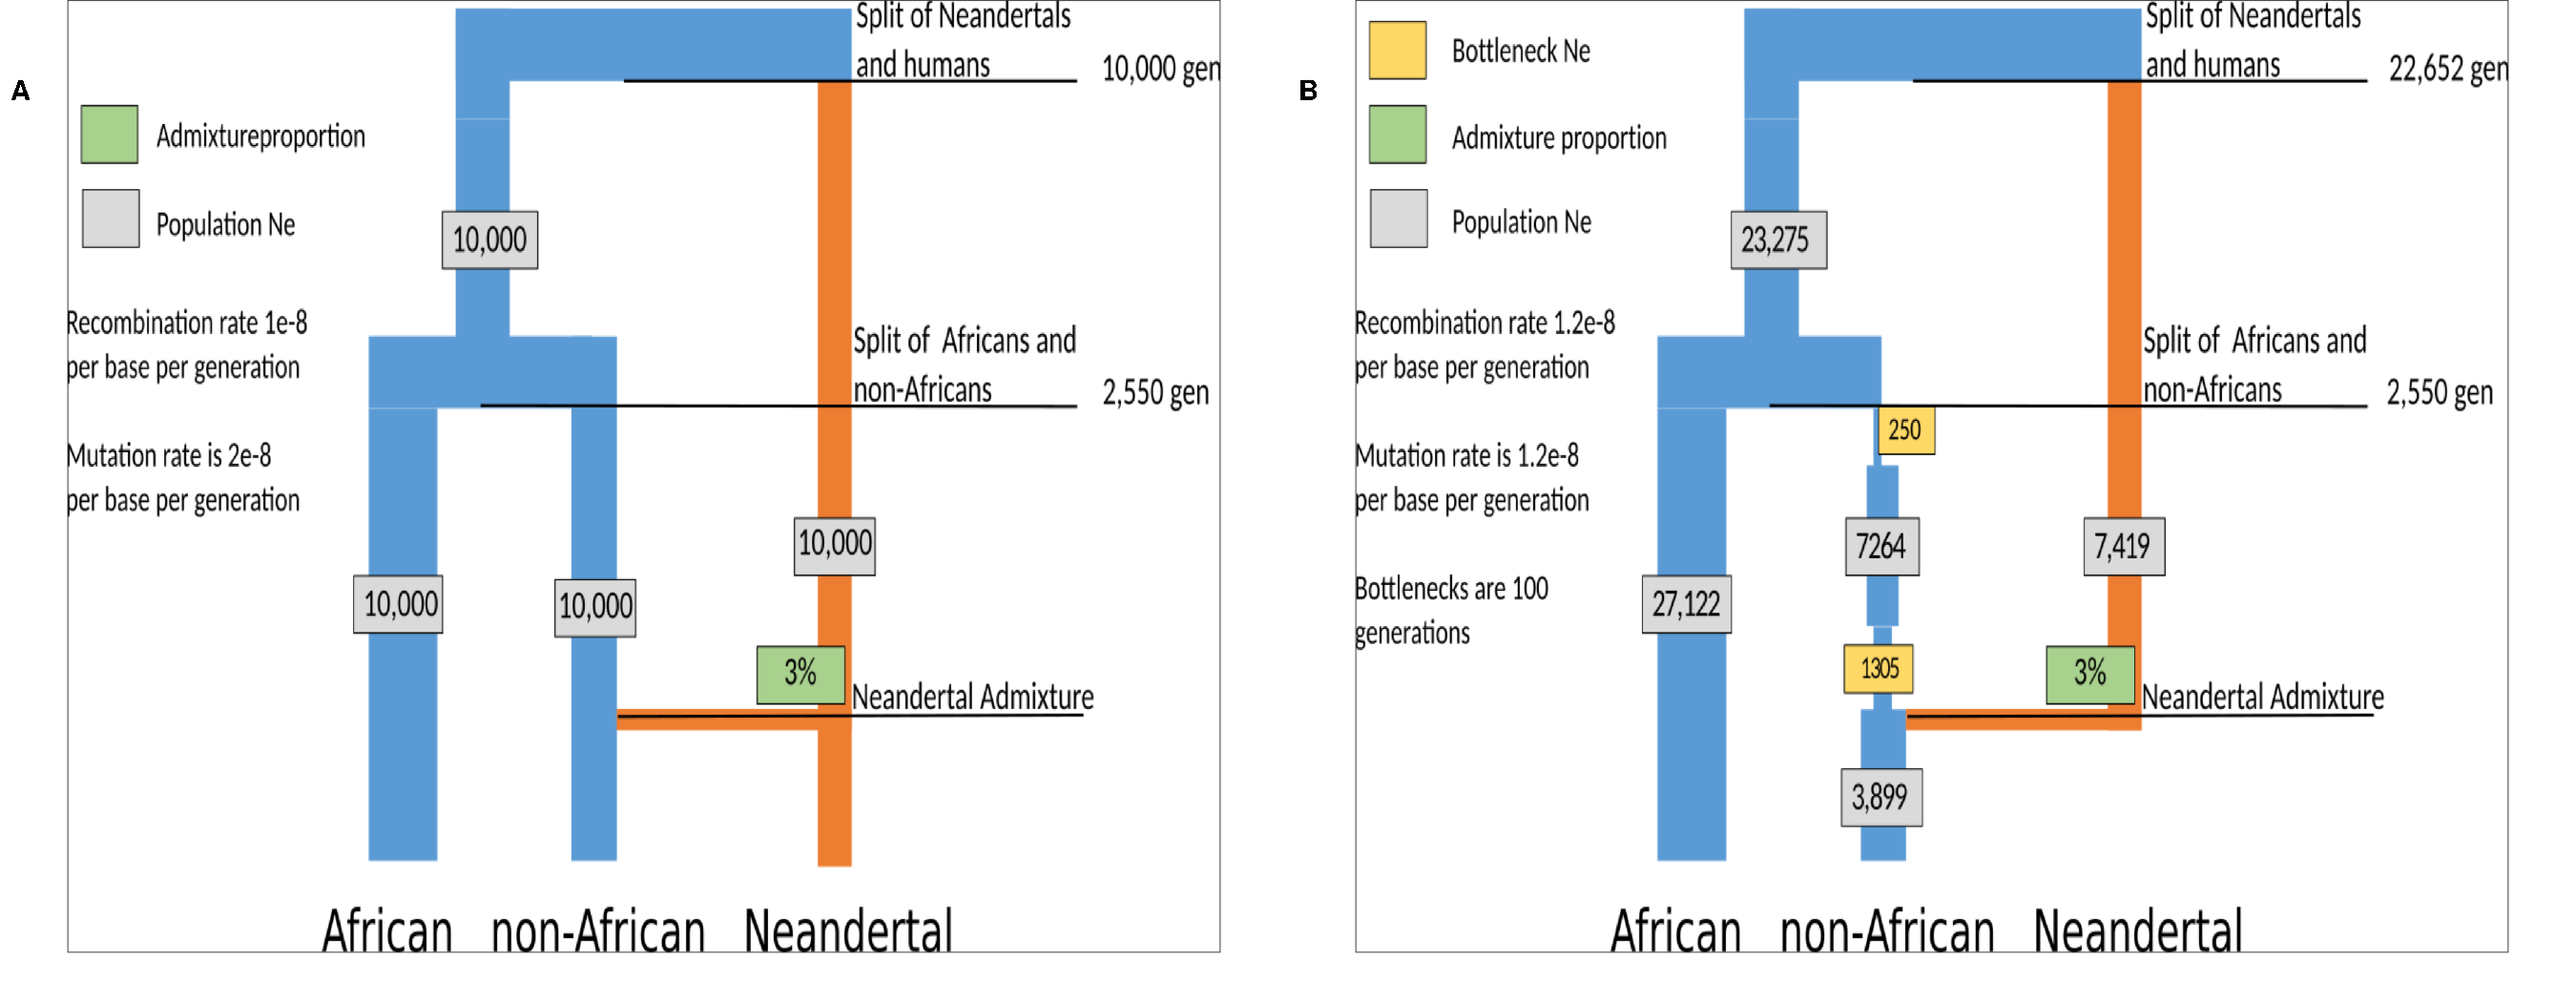
\includegraphics{Admixture_Time_Inference_Paper_Draft_files/figure-latex/Simple_and_Skov.pdf}
\caption{\label{fig:figS1} Demographic models of Neandertal introgression into non-Africans used for the simulations. A) Simple demographic model used for ALD simulations with constant population sizes. B) Complex demographic model with population size changes derived from Skov et al. 2018.}
\end{figure}



\begin{figure}
\centering
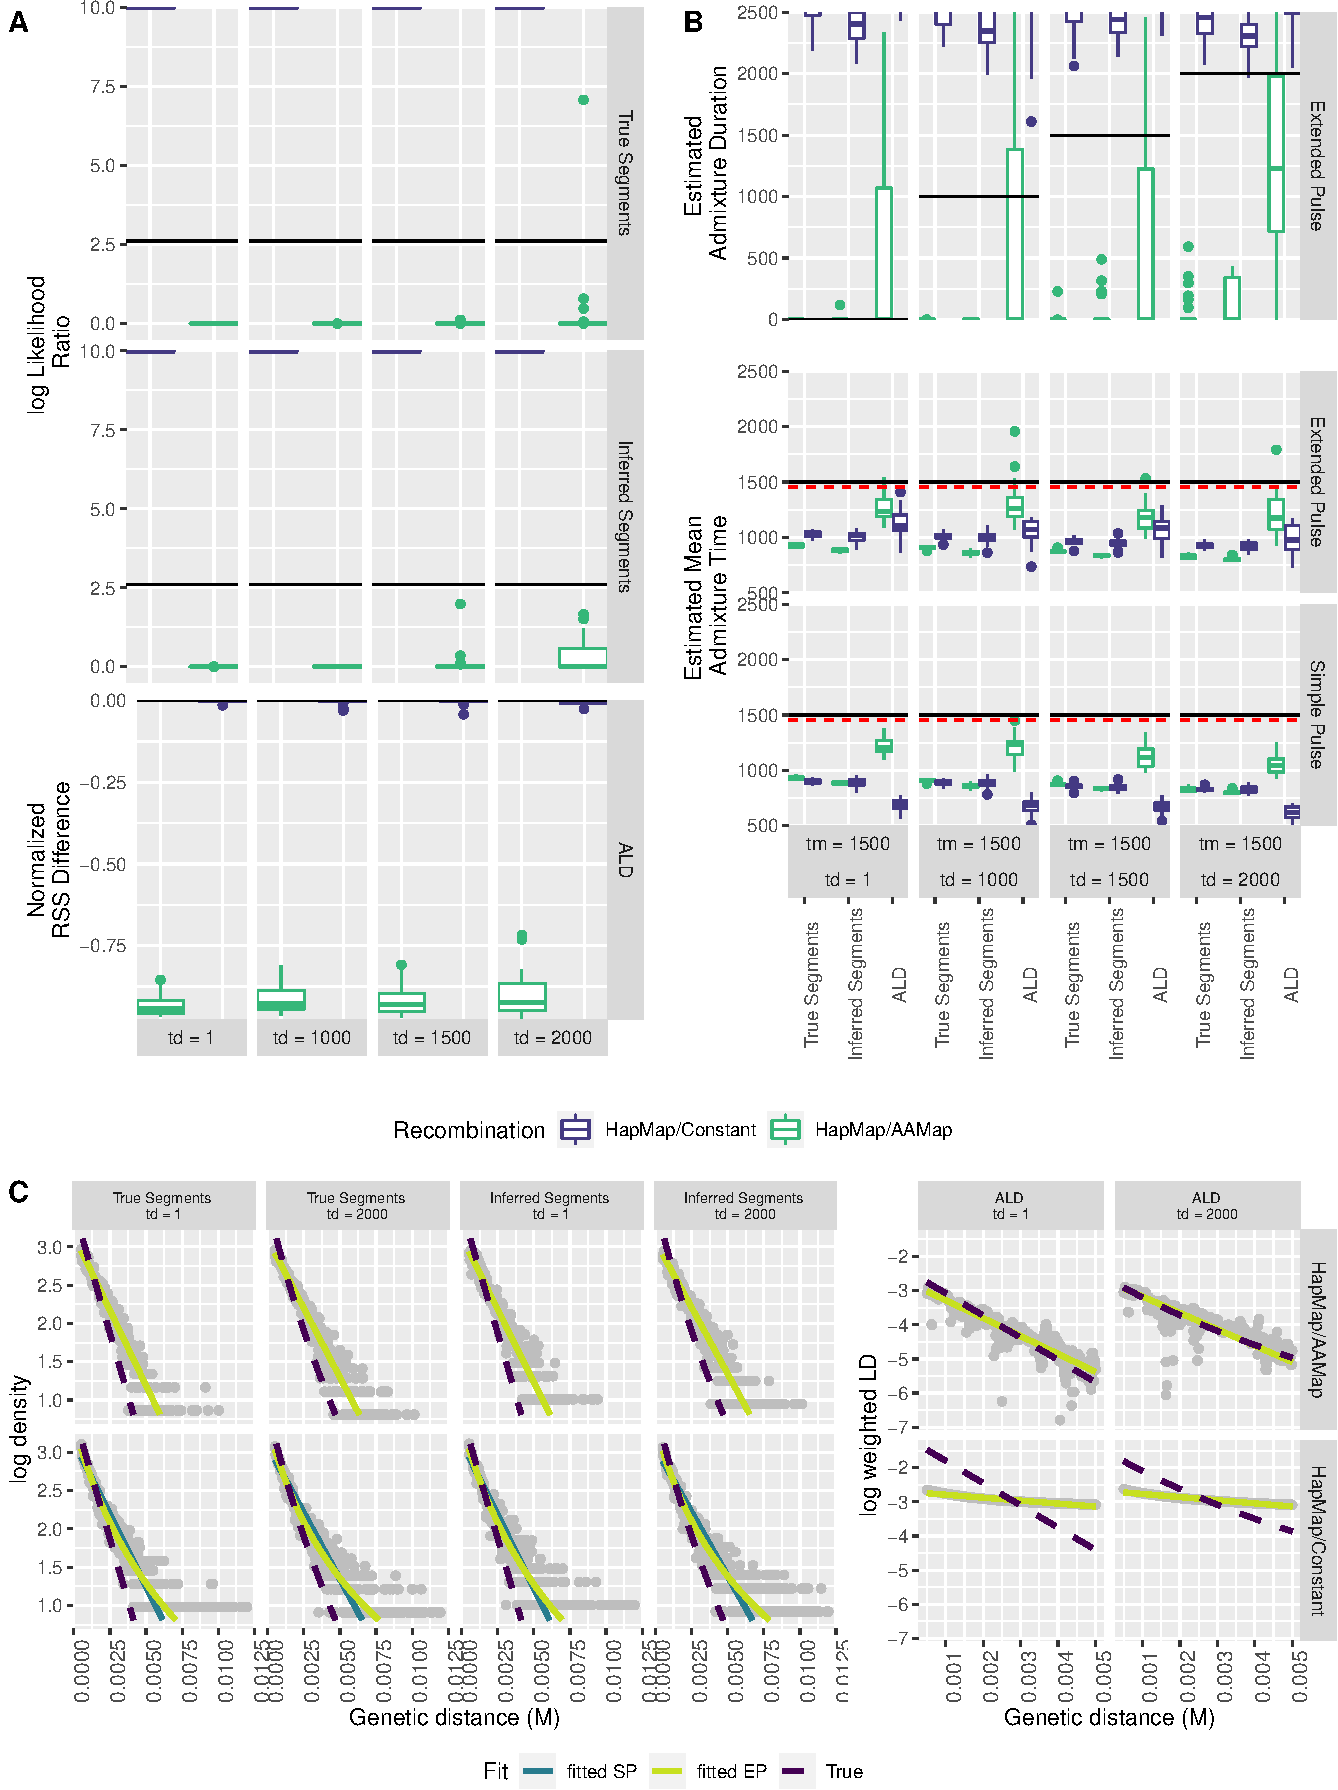
\includegraphics[width=16cm,height=18cm,keepaspectratio]{ATE_Revisions_files/figure-latex/figResult2_all_together_Supplements-1.pdf}
\caption{\label{fig:figResult2_sup} Comparison between the simple and extended pulse one true and inferred segment length and ALD decay estimates using an empirical recombination map (HapMap) for simulations with a fixed mean time ($t_m$) of 1500 generations ago and varying durations ($t_d$). Genetic distances are assigned either using a constant rate or the AAMap . A) log likelihood ratios between the two models for segment data and standardized difference between the residual sum-of-squares between the two models for ALD data. B) Mean time estimates of admixture and extended pulse estimate for admixture duration. Solid black line indicates true $t_m$ and $t_d$, black dotted line indicates expected inverse of the mean segment length under the extended pulse model, red dotted line indicates migration corrected admixture time ($t_m$(1-m)). C) Comparison of the fit to data between the simple and extended pulse using true and estimated parameters. }
\end{figure}



\begin{figure}
\centering
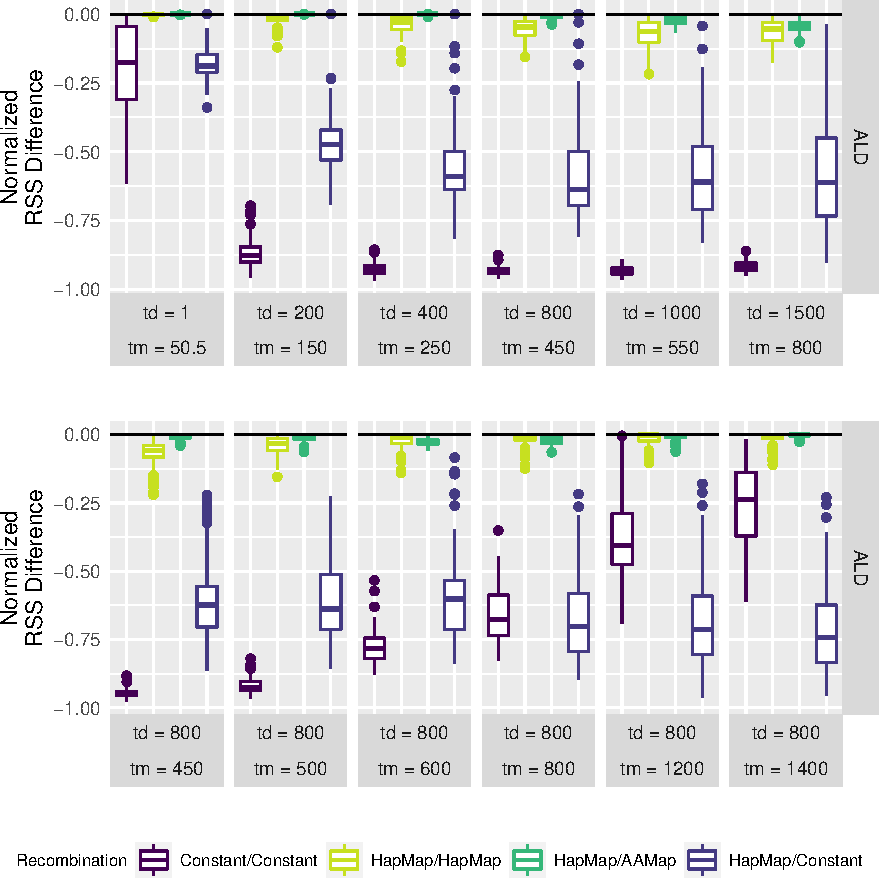
\includegraphics[width=16cm,height=18cm,keepaspectratio]{ATE_Revisions_files/figure-latex/figCloser_Sampling_RSS_Supplement-1.pdf}
\caption{\label{fig:figResult3_4_supplements} Model comparison between the simple and extended pulse  A) All sampled 50 generations after the gene flow ended with different gene flow durations. B)
Different sampling times after 800 generations of gene flow.}
\end{figure}



\begin{figure}
\centering
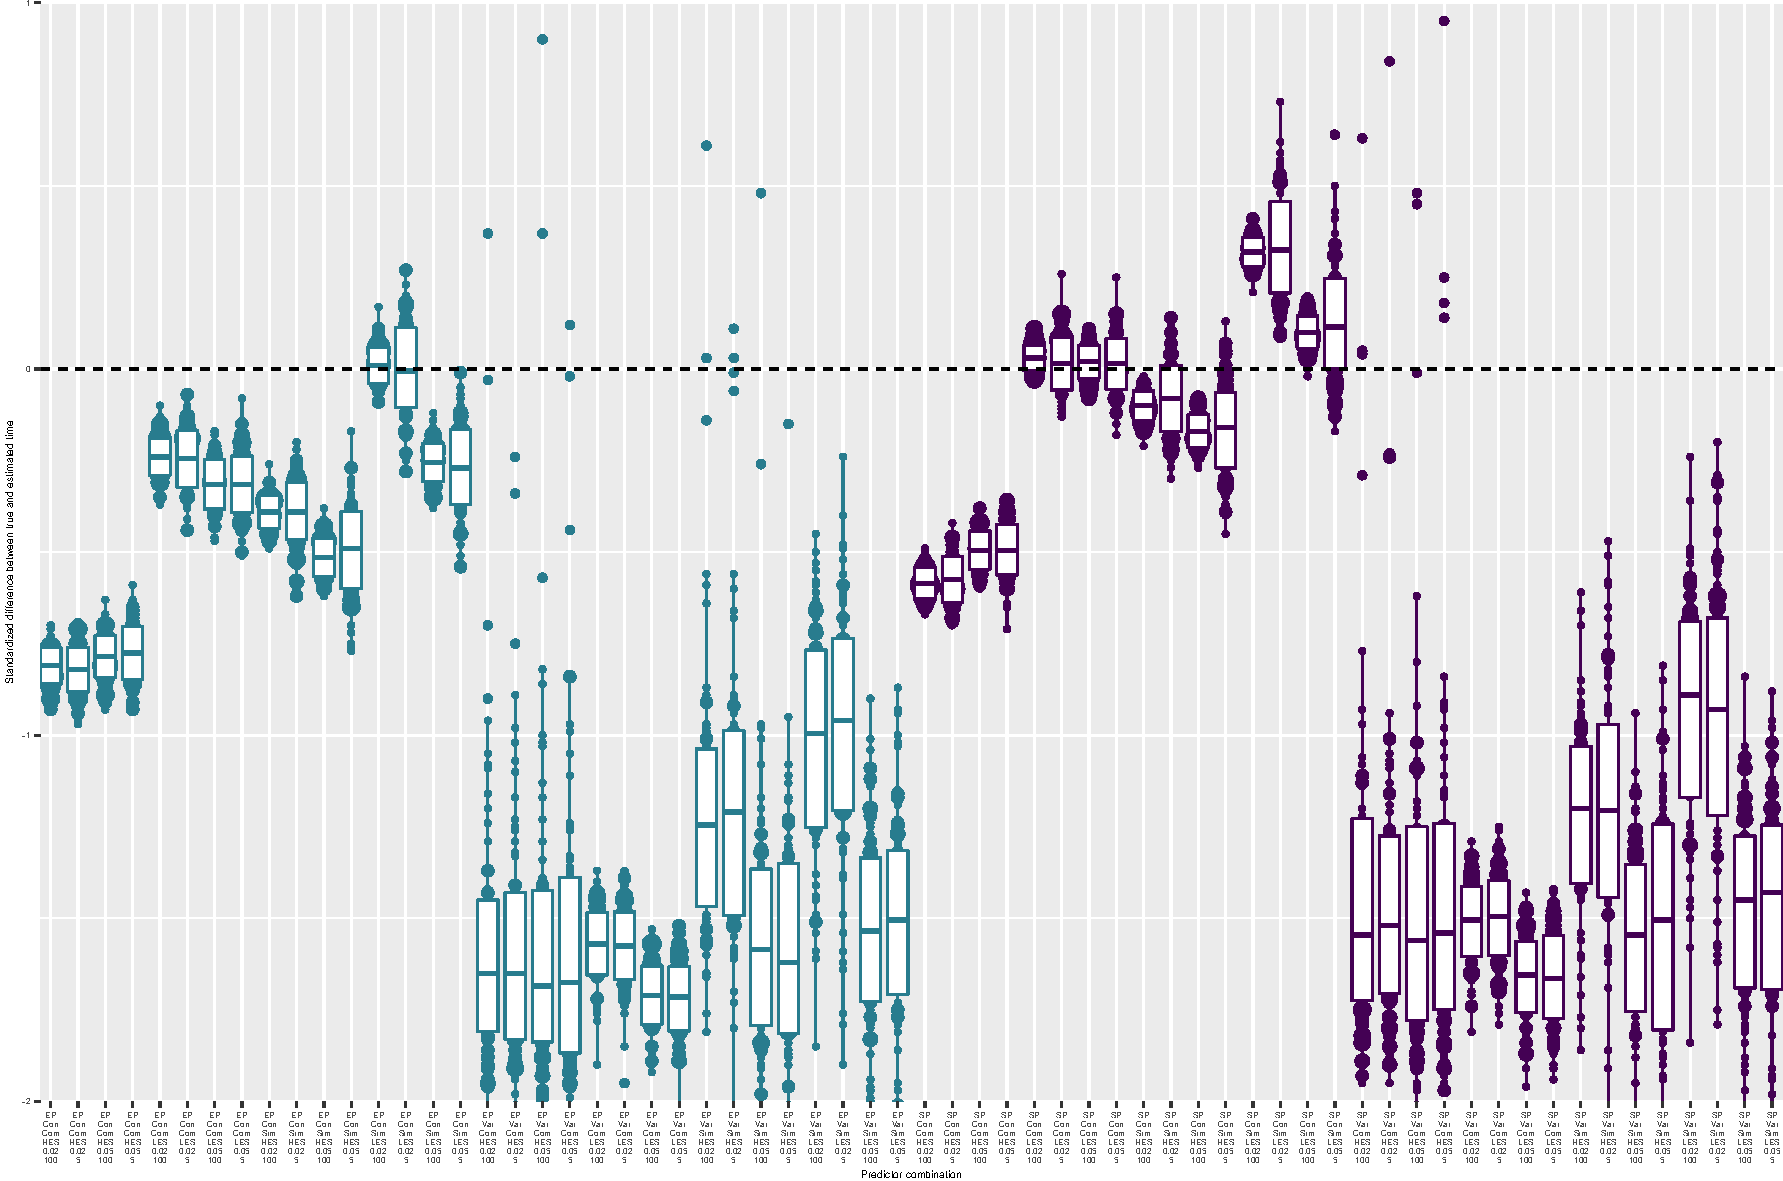
\includegraphics[width=16cm,height=18cm,keepaspectratio]{ATE_Revisions_files/figure-latex/figS2_updated_SP-1.pdf}
\caption{\label{fig:figSGLM_data_SP} Comparison of the standardized difference between true and estimated admixture time for simulations of all combinations of parameters: ascertainment scheme = LES/HES,  $d_{0}$ = 0.02/0.05 cM, demography = simple/complex, recombination = constant/variable, SNP used 100 \% / 5 \% and the gene flow model = simple/extended. Simulations under the simple pulse are indicated in purple, extended pulse in turquoise. Each simulation was repeated 100 times. Dotted horizontal line indicates no difference between true and estimated time.}
\end{figure}

\begin{figure}
\centering
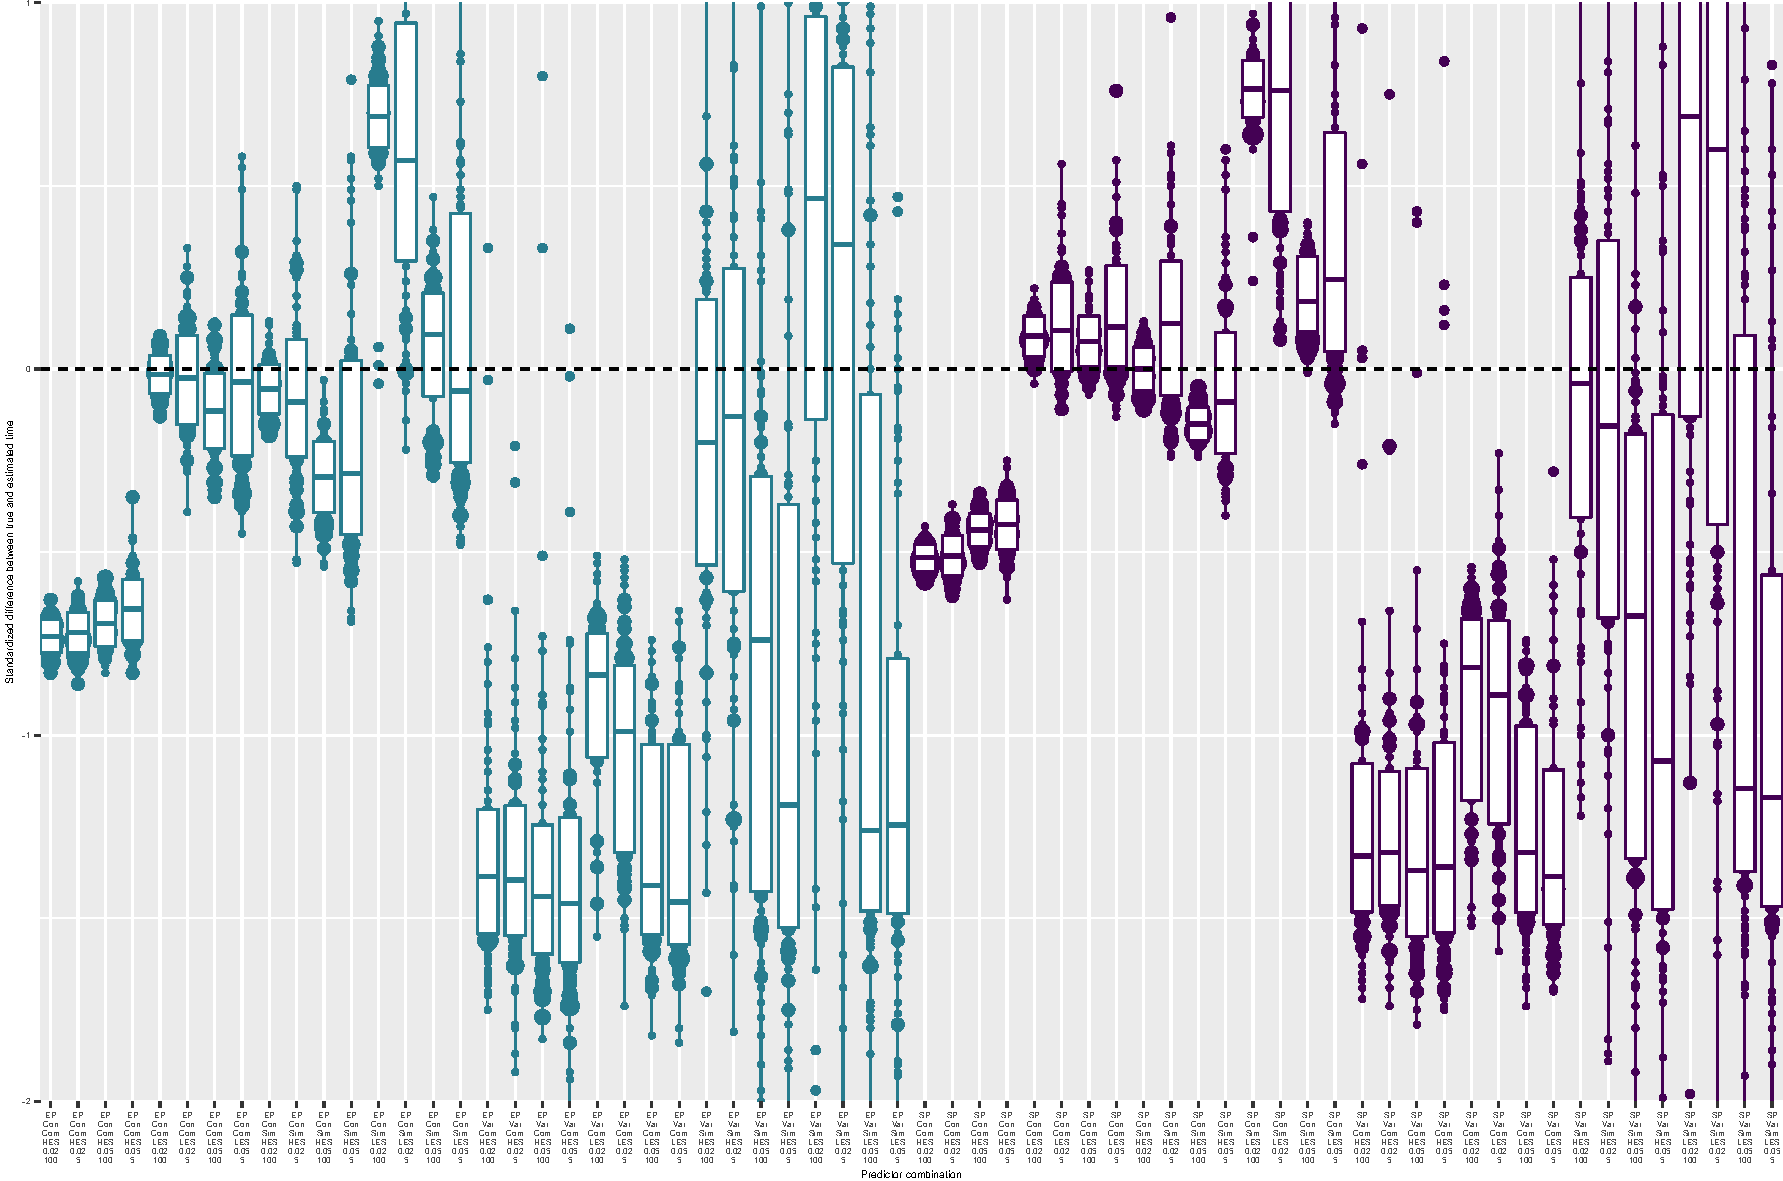
\includegraphics[width=16cm,height=18cm,keepaspectratio]{ATE_Revisions_files/figure-latex/figS2_updated_EP-1.pdf}
\caption{\label{fig:figSGLM_data_EP} Comparison of the standardized difference between true and estimated admixture time for simulations of all combinations of parameters: ascertainment scheme = LES/HES,  $d_{0}$ = 0.02/0.05 cM, demography = simple/complex, recombination = constant/variable, SNP used 100 \% / 5 \% and the gene flow model = simple/extended. Simulations under the simple pulse are indicated in purple, extended pulse in turquoise. Each simulation was repeated 100 times. Dotted horizontal line indicates no difference between true and estimated time.}
\end{figure}

\section{Supplement Tables}


\begin{table}[H]

\caption{\label{tab:table_Supplements_GLM_EP_SP_tm_effect_size_bias}Mean, Standard deviation, 5.5/94.5 compatibility interval of the posterior distribution for every parameter effect on the standardized difference between true and estimated admixture time.} 
\centering

\begin{tabular}[t]{l|l|l|r|r|r}
\hline
model & GLM & variable & mean & 5.5\% & 94.5\%\\
\hline
 & difference & Standard Model & 0.00 & -0.07 & 0.06\\

 & difference & Extended GF & -0.17 & -0.23 & -0.11\\

 & difference & Varying recombination & -1.22 & -1.29 & -1.16\\

 & difference & Complex Demography & -0.28 & -0.34 & -0.21\\

 & difference & d0 = 0.02 & 0.14 & 0.08 & 0.20\\

 & difference & HES & -0.16 & -0.22 & -0.09\\

 & difference & downsampled & -0.01 & -0.07 & 0.06\\

 & difference & Interaction downsampled/HES & -0.15 & -0.21 & -0.08\\

 & difference & Interaction Complex D./Varying R. & -1.28 & -1.35 & -1.19\\

 & difference & Interaction d0 = 0.02/HES & -0.15 & -0.21 & -0.09\\

\multirow{-11}{*}{\raggedright\arraybackslash Simple Pulse} & difference & Interaction d0 = 0.02/Varying R. & -0.89 & -0.96 & -0.83\\
\cline{1-6}
 & difference & Standard Model & 0.21 & 0.14 & 0.27\\

 & difference & Extended GF & 0.10 & 0.04 & 0.16\\

 & difference & Varying recombination & -0.53 & -0.59 & -0.46\\

 & difference & Complex Demography & -0.22 & -0.29 & -0.16\\

 & difference & d0 = 0.02 & 0.59 & 0.53 & 0.66\\

 & difference & HES & 0.03 & -0.03 & 0.10\\

 & difference & downsampled & 0.17 & 0.10 & 0.23\\

 & difference & Interaction downsampled/HES & 0.04 & -0.03 & 0.10\\

 & difference & Interaction Complex D./Varying R. & -1.00 & -1.09 & -0.92\\

 & difference & Interaction d0 = 0.02/HES & 0.02 & -0.05 & 0.08\\

\multirow{-11}{*}{\raggedright\arraybackslash Extended Pulse tm} & difference & Interaction d0 = 0.02/Varying R. & 0.31 & 0.25 & 0.38\\
\hline
\end{tabular}
\end{table}


\begin{table}[H]

\caption{\label{tab:tableSReadl_data_AIC_RSS} AIC and RSS for the fit  to ALD from the 1k Genome data.}

\centering

\begin{tabular}[t]{l|l|l|r|r|r}
\hline
model & GLM & variable & mean & 5.5\% & 94.5\%\\
\hline
 & abs. difference & Standard Model & 0.08 & 0.02 & 0.14\\

 & abs. difference & Extended GF & 0.23 & 0.17 & 0.29\\

 & abs. difference & Varying recombination & 1.33 & 1.27 & 1.39\\

 & abs. difference & Complex Demography & 0.25 & 0.20 & 0.31\\

 & abs. difference & d0 = 0.02 & 0.02 & -0.04 & 0.08\\

 & abs. difference & HES & 0.26 & 0.20 & 0.32\\

 & abs. difference & downsampled & 0.09 & 0.03 & 0.15\\

 & abs. difference & Interaction downsampled/HES & 0.27 & 0.21 & 0.32\\

 & abs. difference & Interaction Complex D./Varying R. & 1.38 & 1.31 & 1.45\\

 & abs. difference & Interaction d0 = 0.02/HES & 0.29 & 0.23 & 0.35\\

\multirow{-11}{*}{\raggedright\arraybackslash Simple Pulse} & abs. difference & Interaction d0 = 0.02/Varying R. & 1.05 & 0.99 & 1.11\\
\cline{1-6}
 & abs. difference & Standard Model & 0.14 & 0.09 & 0.20\\

 & abs. difference & Extended GF & 0.23 & 0.17 & 0.29\\

 & abs. difference & Varying recombination & 0.97 & 0.91 & 1.02\\

 & abs. difference & Complex Demography & 0.17 & 0.11 & 0.23\\

 & abs. difference & d0 = 0.02 & 0.26 & 0.20 & 0.32\\

 & abs. difference & HES & 0.25 & 0.19 & 0.30\\

 & abs. difference & downsampled & 0.22 & 0.16 & 0.27\\

 & abs. difference & Interaction downsampled/HES & 0.33 & 0.27 & 0.38\\

 & abs. difference & Interaction Complex D./Varying R. & 1.32 & 1.24 & 1.39\\

 & abs. difference & Interaction d0 = 0.02/HES & 0.33 & 0.27 & 0.39\\

\multirow{-11}{*}{\raggedright\arraybackslash Extended Pulse tm} & abs. difference & Interaction d0 = 0.02/Varying R. & 0.67 & 0.61 & 0.73\\
\hline
\end{tabular}
\end{table}


\begin{table}[H]
\caption{\label{tab:tableSReadl_data_AIC_RSS} AIC and RSS for the fit  to ALD from the 1k Genome data.}
\centering
\begin{tabular}[t]{l|l|l|l|l}
\hline
Model & A & $t_m$ & c\\
\hline
Simple Pulse & 0.018 (0.018 - 0.018) & 1541 (1487 - 1598) & 1e-05 (6e-06 - 1.5e-05)\\
\hline
Extended Pulse (td=1) & 0.018 (0.018 - 0.018) & 1541 (1487 - 1598) & 1e-05 (6e-06 - 1.5e-05)\\
\hline
Extended Pulse (td=100) & 0.018 (0.018 - 0.018) & 1541 (1488 - 1599) & 1e-05 (6e-06 - 1.5e-05)\\
\hline
Extended Pulse (td=200) & 0.018 (0.018 - 0.018) & 1543 (1490 - 1601) & 1e-05 (6e-06 - 1.5e-05)\\
\hline
Extended Pulse (td=400) & 0.018 (0.018 - 0.018) & 1552 (1498 - 1610) & 1e-05 (6e-06 - 1.5e-05)\\
\hline
Extended Pulse (td=800) & 0.018 (0.018 - 0.018) & 1586 (1531 - 1646) & 1e-05 (5e-06 1.4e-05)\\
\hline
Extended Pulse (td=1000) & 0.018 (0.018 - 0.018) & 1613 (1557 - 1673) & 9e-06 (5e-06 - 1.3e-05)\\
\hline
Extended Pulse (td=1500) &  0.018 (0.018 - 0.018) & 1713 (1654 - 1777) & 7e-06 (3e-06 - 1.1e-05)\\
\hline
Extended Pulse (td=2000) & 0.018 (0.018 - 0.018) & 1875 (1809 - 1945) & 4e-06 (0 - 8e-06)\\
\hline
Extended Pulse (td=2500) & 0.018 (0.018 - 0.018) & 2129 (2055 - 2208) & -1e-06 (-5e-06 - 4e-06)\\
\hline
\end{tabular}
\end{table}

\begin{table}[H]

\caption{\label{tab:tableSReadl_data_AIC_RSS} AIC and RSS for the fit  to ALD from the 1k Genome data.}
\centering
\begin{tabular}[t]{l|r|r}
\hline
Model & AIC & RSS\\
\hline
Simple Pulse & -44845.31 & 4.33e-05\\
\hline
Extended Pulse (td=1) & -44845.31 & 4.33e-05\\
\hline
Extended Pulse (td=100) & -44846.42 & 4.33e-05\\
\hline
Extended Pulse (td=200) & -44849.73 & 4.32e-05\\
\hline
Extended Pulse (td=400) & -44862.90 & 4.30e-05\\
\hline
Extended Pulse (td=800) & -44914.33 & 4.23e-05\\
\hline
Extended Pulse (td=1000) & -44951.47 & 4.18e-05\\
\hline
Extended Pulse (td=1500) & -45069.45 & 4.01e-05\\
\hline
Extended Pulse (td=2000) & -45200.02 & 3.84e-05\\
\hline
Extended Pulse (td=2500) & -45294.46 & 3.72e-05\\
\hline
\end{tabular}
\end{table}

\end{document}